\chapter{Introduction}
\label{sec:introduction}

This project demonstrates methods for estimating linear parameters obtained from
nonlinear vibration signals. The project also demonstrates methods predicting
the behaviour of identified nonlinear systems. The methods are implemented in a
vibration library.

\section{Why nonlinear modeling}
\label{sec:why-nonl-model}

For nonlinear systems, the superposition and thus invariance of modes and
uniqueness of solutions (e.g. the forced steady state response is dependent on
the initial transient behavior) does no longer hold, and many of the techniques
from linear analysis cannot be used.

Linear system is an exception. If excited hard enough, all system displays some
nonlinear behavior. But often the nonlinearity stems from joints (damping),
contact (stiffness) or geometrical nonlinearities, which is why most of the
literature today treats localized nonlinearity, assuming the location of the
nonlinearity is known.
Another reason for dealing with localized nonlinearities, is that no robust
method for localization exists. In his thesis \textcite{kragh2010a} test different
methods for localizing nonlinearity and concludes that \textit{it was not possible to
obtain consistent localization of the nonlinearities} even for simple structures.

With the introduction of ever lighter structures, exotic materials, high speed
machinery, etc., nonlinear tools are needed to fully understand the dynamics.
Also to determine if nonlinear analysis is indeed needed, since this kind of
analysis requires substantial more effort than linear analysis would do.

For a general introduction to nonlinear dynamics, the textbook by
\textcite{juel2003a} can be used.



\section{Nonlinear system identification?}
\label{sec:nonl-syst-ident}

\textcite{kerschen2006a} proposed to regard the identification of nonlinear
structural models as a progression through three steps: \textit{detection},
\textit{characterization} and \textit{estimation}, as outlined in figure
\ref{fig:ident_process}

The first book on the topic was \autocite{worden2000nonlinearity}, and even
though many new methods has been introduced since then, it still gives a good
introduction to the subject as well as a overview of the common types of
nonlinearities.

A comprehensive review of the development in nonlinear system identification was
given by \autocite{kerschen2006a} and just recently by \autocite{noel2016a}. For
comparison of the many techniques in use, the reader is refereed to these
reviews. In this thesis, alternative techniques will not be mentioned.

%\begin{infobox}]

\begin{figure}[ht!]
  \centering
  \begin{mdframed}
    \begin{enumerate}
    \item Detection: {\textit Is there?}\\
      Ascertain if nonlinearity exist in the structural behavior, e.g. yes or
      no.
    \item Characterisation: {\textit Where, what and how?}
      \begin{itemize}
      \item Localize the nonlinearity, e.g. at the joint
      \item Determine the type of nonlinearity e.g.  Coulomb friction\\
        More general: is it stiffness or damping nonlinearity or both. In the
        case of stiffness: is it hardening or softening
      \item Select the functional form of the nonlinearity, e.g.
        $f(x,\dot x) = c \sign (\dot y)$
      \end{itemize}
    \item Parameter estimation: {\textit How much?}\\
      Calculate the coefficients of the nonlinearity model, e.g. $c = 5.47$.\\
      (Ideally the uncertainty should be quantified, e.g. in a probabilistic
      sense, $c \sim N(5.47,1)$. But that is a very difficult task and not
      within the scope of this thesis)
    \end{enumerate}
  \end{mdframed}
  \caption{Identification process for nonlinear structural models}
  \label{fig:ident_process}
\end{figure}

% \end{infobox}


\subsection{Detection}

Of the three steps, detection is the easiest. During test, the structure should
be excited by a sine-sweep and a mere visual inspection of the time series will
show if nonlinearity is present. Signs includes skewness of the envelope,
discontinuity, jumps and lack of invariance with increasing force level. The
excitation level needs to be at an amplitude where the nonlinearity is
activated.

Random excitation is in general not useful, as the randomness of the amplitude
and phase of the excitation creates \textit{linearized} frequency response functions
(FRFs). At least multiple test with different rms levels are required, and still
then it might be difficult to excite the nonlinearities, since the total power
of the input spectrum is spread over the band-limited frequency range used.

The use of impact excitation, as often used in linear analysis, suffers from the
same problems as random excitation. That is, the input is a broad spectrum and
the energy associated with each frequency is low.


Formal methods for detection includes

\begin{itemize}
\item Homogeneity check \\
  Comparing the response of two sweeps with different forcing and calculating
  the cross correlation. It is a test of superposition, by testing if the two FRFs
  normalized with forcing overlay as they will for linear systems.
\item (ordinary) Coherence function \\
  The coherence function compares power spectral densities (PSDs) and are
  required to be unity for all accessible frequencies for the system to be
  linear \textit{and} free of noise. The advantage is that only one test is needed,
  but the method does not distinguish between cases of noise and
  nonlinearity. Instead it is recommend do use:
\item Hilbert transforms \\
  This method detects nonlinearity by doing a Hilbert transform of the FRF,
  which is invariant for a linear FRF.
  A Hilbert transform also only requires one data set and is more sensitive to
  nonlinearity than the coherence function, but still reasonable easy to
  implement. \textcite{kragh2010a} shows that the homogeneity check is superior to
  the Hilbert transforms, having higher sensitivity to nonlinearity.
% \item Wavelet transforms \\
%   Maps a time-history to a time-frequency representation. Fourier transform
%   cannot be used, since it is a one-to-one transformation from time to frequency
%   domain.
\end{itemize}

For all of these methods it is a requirement that the nonlinearities are
activated, e.g. the forcing level end frequency interval should be chosen
adequately. Also, the methods are better at detecting nonlinear stiffness than
nonlinear damping. This is due to the fact that the resonance peak is not
shifted as with the stiffness nonlinearity case. Since the FRF is not shifted
but only lowered, the cross correlation coefficient will not decrease as much as
in the stiffness nonlinearity case. In general damping nonlinearity is difficult
to identify and will only be touched briefly in this thesis.

\subsection{Characterisation}
\label{sec:characterization}

The second step is the most important and also the most difficult, when
localization is not considered.
This step seeks to identify the aspects of the motion that drives the
nonlinearity, e.g. displacement or velocity and a representative functional form
to represent the nonlinearity.


The most used technique is the restoring force surface(RFS). The RFS
provides information of restoring force in the excited range. To visualize the
functional of the restoring force and the dissipative force, two slices in the
RFS is made: at zero displacement and zero velocity. The functional form is then
found by simple inspection of the slices or fitting polynomials and perform
goodness of fit.

Another characterisation method, the Morlet wavelet transform, is used to
visualise how the frequency content changes with amplitude, a consequence of the
energy-frequency dependency for nonlinear vibrations. The visualised
instantaneous spectrum can both be used for detection of nonlinearity and help
estimating the type of nonlinearity,

% Other characterization methods include blackbox modeling, which do
% characterization without regards to the underlying physics, instead using a rich
% and flexible mathematical structure to capture all relevant dynamics.


\subsection{Estimation}
\label{sec:estimation}

The RFS method can be used for estimation as well, fitting the functional form
to the surface. But in order to scale the RFS correct, an estimate of the mass
(or inertia) is needed or the full EOM has to be assembled. This is often
difficult for MDOF systems.

A newer method, introduced by \autocite{noel2013a}, is the frequency-domain
nonlinear subspace identification(FNSI). This method works on
time series exclusive and is able to estimate nonlinear parameters and the
underlying frequency response function(FRF).

% Frequency domain
% methods should generally be less sensitive to noise than time domain
% methods. {\bf men den har jeg ikke skimmet endnu. Det skulle være en lovende
%   metode}


% the parameter estimation is found  The technique requires the measurement devices (accelerometers) to be
% places as close to the nonlinearities as possible.  As already stated, the RFS
% can only estimate parameters within the excited regime.



\section{Beyond nonlinear system identification}
\label{sec:beyond-nonl-syst}

When the identification steps is completed, a structural model can be build from
a FEM of the underlying linear structure with the identified nonlinearities
incorporated. It shall be thought of as (larger) chunks of linear sections
connected through nonlinear elements. To reduce the computational time, the
linear model is often reduced using the Craig-Bampton reduction technique
\autocite{craig1968a}.

If the predictions from the nonlinear FEM can be verified by the
experimental results, the numerical model can be used to \textit{get further
  understanding of the nonlinear dynamics}. The latter is the whole goal of the
identification, as it allows for uncovering new nonlinear regimes of motion and
to make design modifications. The concept of using numerical experiments to
assist with the design is referred to as \textit{virtual prototyping}.


\subsection{Internal resonance}
\label{sec:internal-resonance}


Nonlinear resonances are investigated using an extension of linear normal modes
(LNMs) to nonlinear theory, the nonlinear normal modes (NNMs) described in
section \ref{sec:nonl-norm-modes}.
Where a LNM is interpreted as the deformation along the axis of the vibrating
structure or the rotation, a NNM does not have such a clear interpretation.
An NNM is said to be a periodic oscillation of the underlaying undamped and
unforced nonlinear system and depends on the frequency and energy of the
system. NNMs are described in depth in \autocites{kerschen2009b, kerschen2009a}.


\subsection{Bifurcation}
\label{sec:bifurcation}


Using the HB method, nonlinear forced response curves(NFRCs) for a periodic
excitation are calculated. The transition from a stable periodic solution to an
unstable solution occurs through bifurcations. The type of bifurcation is used
to qualify the type of unstable solution emerging. The HB method followed here
were introduced in \autocite{detroux2015a}.

% , following the outline in


\section{Thesis outline}
\label{sec:thesis-outline}

To summarise, chapter 2 introduces the wavelet transform and RFS for
characterisation and FNSI for estimation; the methods used for identification as
depicted in fig. \ref{fig:ident_process}. All methods are working exclusively on
time series.

Chapter 3 introduces numerical methods working on a finite element
discretization of the identified system. These methods are used to get
qualitative information on the nonlinear behavior.

Chapter 4 introduce the python library implementing the methods and gives a
brief example on how to use it. All examples from this thesis can be found
online together with the library.

In chapter 5 the methods from chapter 2 and 3 are demonstrated on two nonlinear
systems.

All methods are exemplified on the nonlinear two degree of freedom system(2DOF)
\eqref{eq:2dof} presented next.



\section{Numerical example}
\label{sec:numerical-example}


To illustrate the methods presented, the 2-DOF system shown in figure
\ref{fig:duf_schematic} is used throughout the thesis. It will be referred to as
the coupled duffing system, with parameters listed in table \ref{tab:duf_par}
and natural frequencies and damping ratio for the two modes listed in table
\ref{tab:duf_eigen}. The equations of motion are

\begin{equation}
  \label{eq:2dof}
  \begin{aligned}
    &m_1\ddot x_1 + c \dot x_1 + kx_1 + \mu x_1^3 + d(x_1 - x_2) = p \\
    &m_2\ddot x_2 + c \dot x_2 + kx_2 + \mu x_2^3 + d(x_2 - x_1) = 0 \\
  \end{aligned}
\end{equation}
where $x_1,x_2, p$ all depends on time.

An example on how a real continous beam with different nonlinear boundary
conditions is transformed into a coupled MDOF nonlinear duffing oscillator is
given in \textcite{mhermansen2017a}


\begin{center}
  \begin{tabular}{*{6}{c}}
    \hline
    $m_1$ (kg) & $m_2$ (kg) & $k$ (N/m) & $d$ (N/m) & $c$ (N/ms) & $\mu$ (N/$m^3$) \\
    1 & 1 & 1 & 5 & 0.1 & 1 \\
    \hline
  \end{tabular}
  \captionof{table}{Linear and nonlinear parameters for the coupled Duffing
    system}
  \label{tab:duf_par}
\end{center}


\begin{center}
  \begin{tabular}{*{3}{c}}
    \hline
    Mode & Frequency (rad/s) & Damping ratio (\%) \\
    1 & 1.00 & 5.00 \\
    2 & 3.32 & 1.51 \\
    \hline
  \end{tabular}
  \captionof{table}{Linear natural frequencies and damping ratios for the
    coupled Duffing system}
  \label{tab:duf_eigen}
\end{center}


\begin{figure}[!ht]
  \centering
  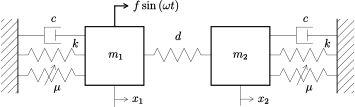
\includegraphics[width=0.5\linewidth]{2dof_duffing/2dof_duffing}
  \caption{Schematic representation of the coupled duffing system}
  \label{fig:duf_schematic}
\end{figure}

For generating data for characterisation with WT and RFS, the system is
simulated using a logarithmic sine sweep with a sweep rate of 1 oct/min.

For identification, a single band-limited (0-15 rad/s) normally distributed
random signal with 5000 points repeated 9 times and a root mean square(rms)
value of 3N is used. This signal is called a multisine. The frequencies are
chosen to include third harmonics of the highest natural frequency.

Formally a multisine is defined as a \textit{sum of sine waves with related
  frequencies}\autocite{overschee1996a}:

\begin{equation}
  \label{eq:multisine}
  u(t) = N^{1/2} \sum_{-N/2+1}^{N/2-1} U_k e^{j \left( 2\pi k \frac{f_s}{N}t + \phi_k \right)}
\end{equation}
where $N$ is the number of time sample and $f_s$ the sampling frequency. The
phases $\phi_k$ are drawn from a uniform distribution on $[0, 2\pi[$ and the
amplitudes $U_k$ are controlled to create the desired spectrum(normally flat in
the desired frequency spectrum). The signal $u$ is asymptotically normally
distributed as $N$ tends to infinity.


%%% Local Variables:
%%% mode: latex
%%% TeX-master: "../report"
%%% End:
